\documentclass[11pt]{article}
\usepackage[margin=1in]{geometry}
\usepackage[T1]{fontenc}
\usepackage{lmodern,microtype,amsmath,amssymb,amsthm,mathtools}
\usepackage{graphicx,booktabs,array,longtable,float}
\usepackage{tikz}
\usetikzlibrary{arrows.meta,positioning}
\usepackage[numbers,sort&compress]{natbib}
\usepackage[colorlinks=true,linkcolor=blue,citecolor=blue,urlcolor=blue]{hyperref}
\usepackage{enumitem}
\hypersetup{pdftitle={Reliable productive operation of coupled autocatalytic reactors under mechanistic refinement},pdfauthor={}}
\setlength{\emergencystretch}{2em}\allowdisplaybreaks[1]
\setlist{nosep}
\newtheorem{theorem}{Theorem}
\newtheorem{lemma}[theorem]{Lemma}
\newtheorem{proposition}[theorem]{Proposition}
\newtheorem{corollary}[theorem]{Corollary}
\theoremstyle{definition}\newtheorem{definition}[theorem]{Definition}
\newcommand{\R}{\mathbb R}
\newcommand{\N}{\mathbb N}
\newcommand{\Ready}{\mathsf{Ready}}
\newcommand{\Law}{\mathbb P}
\newcommand{\dd}{\,\mathrm dt}
\newcommand{\diag}{\operatorname{diag}}
\newcommand{\code}[1]{\texttt{\small #1}}
\title{Reliable productive operation of coupled autocatalytic reactors under mechanistic refinement}
\author{}
\date{17 September 2026}
\begin{document}
\maketitle
\begin{abstract}
When does a chemical reactor retain useful operation after it is coupled to other
reactors and an effective reaction is replaced by an explicit intermediate mechanism?
For a specified reversible autocatalytic exporter, we prove a finite-mission guarantee
that includes recovery after molecular withdrawal, loss and refill, collected product,
food input and gross reaction service. On a symmetric exchange graph with $n$ reactors,
weighted degree at most $\Delta$ and integer count scale $V\ge10^4$, the seven-species
refinement completes $m$ cycles with probability at least
$\max\{0,1-29nm\exp[-V/(2\cdot10^{12}(1+\Delta)^3)]\}$.
Policies may use the complete history of returned states and physical counters.
An exact material-forced reduction of the six-species donor explains which information
can be removed; an explicit witness shows why simply deleting the intermediate is not
an exact reduction. The proof controls material, stock and phase separately, then
composes from actual random endpoints. An augmented-inventory identity shows that
every successful mission of at least 55 cycles necessarily produces net new inventory
beyond depletion of its initial supply. A connected two-reactor, 100-cycle instance
has certified success probability above $99\%$. The refined operational results have
Lean-checked proofs; the donor theorem and the additional accounting consequences
are proved conventionally. The count scale is sufficient, not optimized or experimentally calibrated.
\end{abstract}

\section{Introduction}
Structural autocatalysis and reliable production are different mathematical questions.
The RAF framework identifies reaction sets that are reflexively autocatalytic and
food-generated: their catalysts are available from the food set or the set's products,
and their reactants can be built from food using the set's reactions
\citep{hordijk2004}. Such a structural criterion does not by itself specify rates,
washout, a withdrawal protocol or the probability of meeting a product quota.
Here autocatalysis has an explicit kinetic realization: the productive route
$X+U\rightleftarrows C_1$, $C_1+W\rightleftarrows C_2$,
$C_2\rightleftarrows Z$, $Z\rightleftarrows2X$ converts one $X$ into two while
using food. We analyze this specified exporter; we do not infer operation from a
generic RAF classification or identify a particular laboratory chemistry.

Two modifications make operation more demanding. Conservative transport preserves
global material but creates local fluctuations and dependence. Inserting an intermediate
stores material, introduces a washout channel, and separates upstream from downstream
conversion. Existing inheritance results address related but distinct properties.
Feliu and Wiuf relate models with intermediates through steady-state parameter matching
\citep{feliu2013}; Banaji proves preservation of the capacity for nondegenerate
equilibria and periodic orbits under suitable reaction splitting \citep{banaji2023}.
Cappelletti and Wiuf study elimination of intermediates in multiscale stochastic
networks \citep{cappelletti2016}. These results do not directly give the fixed-parameter,
intervention-dependent output and resource event considered here.

Our contribution is a source-specific guarantee for useful operation under both
modifications. Success is defined by actual collected molecules and the actual state
returned after each cycle, rather than by closeness of all trajectories to a donor model.
The principal theorem treats the literal seven-species jump process with an intermediate
lifetime parameter fixed at $\theta=0.01$. A separate local deterministic theorem allows
$0<\theta\le0.01$. The six-species donor provides an exact material-forced reduction
and a conventional network reliability theorem. Neither theorem is obtained by assuming
the intermediate vanishes. The improved exponential constant for the refined source
comes from a less restrictive internal error budget; it is not a comparative claim
that the refined chemistry is intrinsically more reliable.

The argument combines positive material balances, a productive-stock barrier, a short
phase comparison and exponential martingale bounds. The last belong to the general
time-uniform concentration framework \citep{howard2020}; we give the bound and the
source estimates used here. A pathwise inventory telescope then distinguishes sustained
net synthesis from spending initially carried stock. The paper includes the readable
proof and the quantitative estimates required for its conclusions; the accompanying
proof map separates formal checks, conventional deductions and numerical illustrations.

\section{The literal chemistry and intervention}
Write the concentration vector as $c=(u,w,x,c_1,c_2,z,h)\in\R_+^7$,
for species $(U,W,X,C_1,C_2,Z,D)$, and molecular counts as $N=Vc$.
The rows of Table~\ref{tab:chemistry}, indexed $0,\ldots,6$, specify reversible pairs; coefficients multiply the
usual concentration monomial. Every species has unit washout, and $U,W$ each have unit feed.
Let $\epsilon_0=1/(5\cdot10^8)$, $\eta_0=1/(8\cdot10^9)$, $19\le r\le21$, $1/50\le d\le1/25$, and $\beta=1/100$.

\begin{table}[ht]
\centering
\begin{tabular}{lll}
\toprule Pair & Forward coefficient & Reverse coefficient\\\midrule
$U+W\rightleftarrows X$ & $1/(5\cdot10^8)$ & $1/(5\cdot10^9)$\\
$X+U\rightleftarrows C_1$ & $20$ & $20$\\
$C_1+W\rightleftarrows C_2$ & $20$ & $20$\\
$C_2\rightleftarrows Z$ & $20$ & $2$\\
$Z\rightleftarrows 2X$ & $r$ & $r$\\
$X\rightleftarrows D$ & $d(1+\beta)$ & $d\beta/\theta$\\
$D\rightleftarrows U+W$ & $d/\theta$ & $d\eta_0(1+\beta)/\beta$\\
\bottomrule
\end{tabular}
\caption{The seven chemical pairs. Two feeds and seven washouts give 23 local labels.
Gross service counts both directions of $X\rightleftarrows D$.}
\label{tab:chemistry}
\end{table}

The deterministic vector field is $f(c)=(1,1,0,0,0,0,0)-c+\sum_{j=0}^6\nu_j j_j(c)$,
where $\nu_j$ is the product-minus-reactant vector and $j_j$ the net flux of row $j$.
In particular, the two new net fluxes are
\begin{equation}\label{eq:newflux}
j_5=d(1+\beta)x-d\beta h/\theta,\qquad
j_6=dh/\theta-d\eta_0(1+\beta)uw/\beta.
\end{equation}
The intermediate is retained as a state variable at all times, including between cycles.
Define augmented materials, productive stock and product inventory by
\begin{align}
 A&=u+x+2c_1+2c_2+2z+h,\\
 B&=w+x+c_1+2c_2+2z+h,\\
 Y&=x+\tfrac98c_1+\tfrac75c_2+\tfrac95z,\\
 I&=x+c_1+c_2+2z.
\end{align}
For nonnegative states, $I\ge5Y/7$. The gross service rate is
\begin{equation}\label{eq:service}
g(c)=d(1+\beta)x+d\beta h/\theta.
\end{equation}
It is a sum of directional rates, not their net difference.

An intervention chooses $q\in[1/4,3/4]$, survival factors
$\ell_s\in[49/50,1]$ for all seven species, and food errors
$e_U,e_W\in[-1/200,1/200]$. It maps $c_s$ to $q\ell_s c_s$ and then adds
$1-q+e_U$ to $U$ and $1-q+e_W$ to $W$. In the count process each molecule
is independently categorized, conditional on the action and current state, as withdrawn, lost or retained with probabilities
$1-q$, $q(1-\ell_s)$ and $q\ell_s$; the refill is the actual integer floor
$\lfloor V(1-q+e_s)\rfloor$. Choices may differ by compartment and depend on
the available past history.

\begin{definition}
For $\theta>0$, $c\in\Ready(\theta)$ if $c\ge0$ and
\begin{equation}\label{eq:ready}
\frac{159}{160}\le A,B\le\frac{161}{160},\qquad
Y\ge\frac1{20},\qquad h\le\frac{1101}{1000}\theta.
\end{equation}
One cycle consists of the intervention followed by four time units of flow.
The product collection window is $(3,4]$; the food and service accounting window is $(0,4]$,
with refill included separately in food.
\end{definition}

\begin{figure}[ht]
\centering
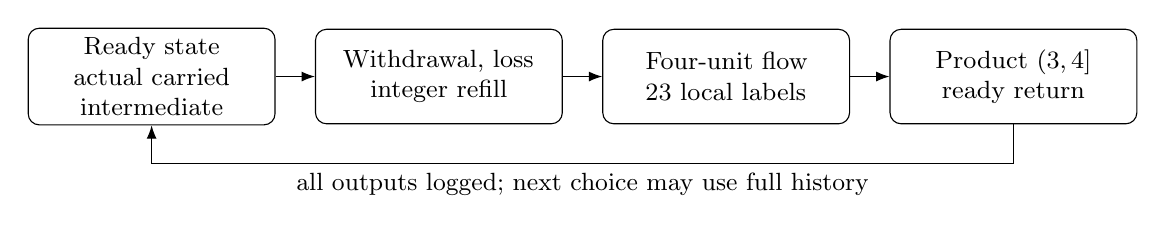
\begin{tikzpicture}[>=Latex, node distance=5mm,
 box/.style={draw,rounded corners,align=center,font=\small,minimum height=12mm,text width=29mm}]
\node[box] (a) {Ready state\\actual carried intermediate};
\node[box,right=of a] (b) {Withdrawal, loss\\integer refill};
\node[box,right=of b] (c) {Four-unit flow\\23 local labels};
\node[box,right=of c] (d) {Product $(3,4]$\\ready return};
\draw[->] (a)--(b);\draw[->] (b)--(c);\draw[->] (c)--(d);
\draw[->] (d.south)--++(0,-.5)-|node[below,pos=.25,font=\small]{all outputs logged; next choice may use full history}(a.south);
\end{tikzpicture}
\caption{The physical cycle. Product marks are existing washout events. Repetition uses the
actual returned state, and failed outcomes remain in the probability law.}
\end{figure}

\subsection{The donor and the common operating contract}
The donor uses the first five pairs of Table~\ref{tab:chemistry}, but replaces its
last two pairs by $X+F\rightleftarrows U+W+P$ with forward and reverse rates
$dx$ and $d\eta_0uw$. The external species $F,P$ have unit maintained activity
and are not internal material coordinates. A compatible bookkeeping realization of
the split rates is $X+F\rightleftarrows D\rightleftarrows U+W+P$; no chemical
potentials or energy costs are assigned here. The donor has 20 local labels: twelve
directed chemical channels, two feeds and six washouts. Define its materials
$A_0=u+x+2c_1+2c_2+2z$, $B_0=w+x+c_1+2c_2+2z$. Its ready set has the same
material interval and stock floor as \eqref{eq:ready}, with $A_0,B_0$ replacing
$A,B$ and no intermediate constraint. Its service counts both directions of its
single driven pair. All other pulse, collection and food conventions are the same.
For either process, jumps at a fixed positive time have probability zero, so the
donor convention $[3,4]$ and the adopted $(3,4]$ define the same event almost surely.
The latter convention is used for the literal refined marked law.

\pagebreak[3]
\section{Operational theorems}
\begin{theorem}[Local deterministic repeated operation]\label{thm:det}
Fix $\beta=1/100$, $0<\theta\le1/100$ and the stated $r,d$ ranges.
From any state in $\Ready(\theta)$, every sequence of admissible interventions,
chosen from the cycle index and current state, admits successive nonnegative global
solutions of the literal seven-species ODE. Every four-unit endpoint is in
$\Ready(\theta)$. In each cycle, stock is at least $1/20$ for $t\ge5/2$, and
\begin{equation}\label{eq:detoutputs}
\int_3^4 I\dd\ge\frac1{28},\quad
\int_3^4 x\dd\ge\frac1{540},\quad
\int_0^4 g\dd\le\frac{112201}{625000}.
\end{equation}
Each food account, including refill, is at most $951/200$ per cycle.
Consequently all these inequalities sum over every finite prefix of cycles.
\end{theorem}

For the stochastic statement take $\theta=\beta=1/100$. There are $n>0$ compartments,
with rates $r_i,d_i$ in the same ranges. A nonnegative symmetric matrix $k$ with $k_{ii}=0$ acts on every
species by molecule exchange: a molecule of species $s$ moves from $i$ to $j$ at total
rate $k_{ij}N_{i,s}$. Assume $\sum_j k_{ij}\le\Delta$, $\Delta\ge0$. Write
\[
(\mathcal D a)_i=\sum_j k_{ij}(a_j-a_i).
\]
The exchange is nonselective and the count scale is the same at every node.
For a reaction with consumption vector $a$, production vector $b$ and coefficient $\kappa$,
its propensity at a count state is
\begin{equation}\label{eq:propensity}
\lambda(N)=\kappa V\prod_s\frac{(N_s)_{a_s}}{V^{a_s}},
\qquad (N)_a=N(N-1)\cdots(N-a+1).
\end{equation}
The jump is $N-a+b$ when enabled; disabled channels have rate zero.
In particular, $2X\to Z$ has propensity $rN_X(N_X-1)/V$, with no factorial divisor.
Each food feed has rate $V$, and each washout label has rate $N_s$.
These propensities define the continuous-time Markov reaction law through exponential
holding times and rate-proportional reaction choices \citep{gillespie1977}.

Let $Q_I,Q_X$ be the natural-number product marks in $(3,4]$.
Washout of $X,C_1,C_2,Z$ contributes respectively $1,1,1,2$ to $Q_I$;
only washout of $X$ contributes to $Q_X$. Let $F_U,F_W$ include continuous food arrivals
and pulse refill. Let $G$ count both directions of $X\rightleftarrows D$ in $(0,4]$.
Intermediate washout is not a product mark.

\begin{theorem}[Finite-count mission]\label{thm:mission}
Let $m\in\N$, $V\in\N$, $V\ge10000$, and let every initial compartment be ready after normalization
by $V$. Under the unrestricted literal pulse-plus-flow law, every admissible controller
on the history of returned states and counters satisfies
\begin{equation}\label{eq:mission}
\Law(\hbox{all $m$ cycles succeed})\ \ge\
\max\left\{0,1-29nm\exp\left(-\frac{V}{2\cdot10^{12}(1+\Delta)^3}\right)\right\}.
\end{equation}
Success means that, in every compartment and cycle, the actual endpoint is in
$\Ready(1/100)$ and
\begin{equation}\label{eq:integer}
Q_I\ge\lceil V/56\rceil,\quad Q_X\ge\lceil V/1080\rceil,\quad
F_U,F_W\le5V,\quad G\le\lfloor V/5\rfloor.
\end{equation}
The same bound holds on any measurable history space whose next observed output has
the literal pulse-plus-flow conditional law, whose current counts equal that observed
return, and whose log appends the actual output.
\end{theorem}

The history assumptions in the last sentence specify a model interface; they do not
assume a success probability. A normalized history kernel for arbitrary policies on all
previous returned states and counters is explicitly constructed. Richer observations
are covered when their conditional law satisfies the stated interface. No independence
between nodes or successive cycles is required.

\begin{theorem}[Coupled donor operation]\label{thm:donor}
For the six-species donor, $V\ge10000$, the stated graph and rate assumptions,
and initial readiness at every node, all $m$ cycles meet the common integer
contract with probability at least
\[
\max\{0,1-27nm\exp[-V/(2\cdot10^{14}(1+\Delta)^3)]\}.
\]
The controller may use the actual joint past. This theorem has a conventional
proof; Appendix~\ref{app:donor} supplies its source estimates and probability budget.
\end{theorem}

\begin{corollary}[Sizing and yield]\label{cor:sizing}
For $m\ge1$ and $0<\delta<1$, it suffices that
\begin{equation}
V\ge \max\left\{10000,\ 2\cdot10^{12}(1+\Delta)^3
             \log\frac{29nm}{\delta}\right\}
\end{equation}
to guarantee mission probability at least $1-\delta$.
On the success event, the division-free food-to-product inequalities
\begin{equation}\label{eq:yield}
F_U+F_W\le560Q_I,\qquad F_U+F_W\le10800Q_X
\end{equation}
hold per compartment per cycle, and hence after summing over any successful mission.
\end{corollary}
\begin{proof}
Exponentiation of the sizing inequality bounds the error term in
\eqref{eq:mission} by $\delta$. Also $F_U+F_W\le10V$, while
$Q_I\ge V/56$ and $Q_X\ge V/1080$. These comparisons do not divide by a random output.
\end{proof}

For a concrete connected example take two nodes, $k_{12}=k_{21}=1$, zero diagonal,
and $V=224000000000000$. Choose initial normalized states
\begin{equation}\label{eq:seeds}
c^{(1)}=(19/20,19/20,1/20,0,0,0,0),\quad
c^{(2)}=(13/14,13/14,0,0,1/28,0,0).
\end{equation}
Both count vectors are integral at this $V$ and ready. For $m=100$, the proved lower
bound is $1-5800e^{-14}>0.99$. A rational Taylor certificate
$e^{14}\ge600000$ is sufficient to verify the strict inequality. The scale is sufficient,
not claimed minimal.

\begin{figure}[ht]
\centering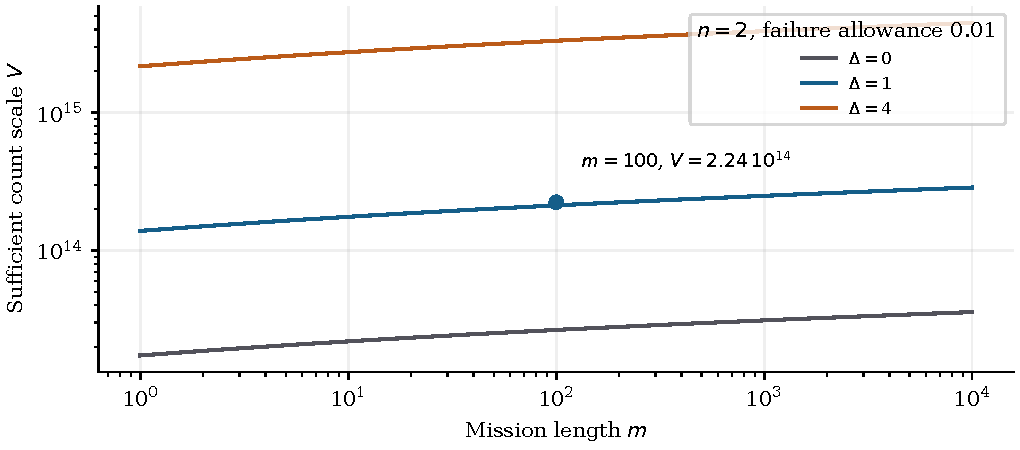
\includegraphics[width=.94\linewidth]{figures/scale.pdf}
\caption{The certified sufficient scale from Corollary~\ref{cor:sizing}. The dot is the
connected 100-cycle instance. Curves describe a theorem bound, not empirical failure
probabilities or calibrated molecule requirements.}\label{fig:scale}
\end{figure}

\section{Material closure and the role of the intermediate}\label{sec:reduction}
\begin{proposition}[Exact material-forced donor reduction]\label{prop:reduction}
On each deterministic flow segment, the donor is equivalent to the four phase
equations for $(x,c_1,c_2,z)$ supplied with
\begin{align}
A_0(t)&=\mathbf1+e^{-t}e^{t\mathcal D}(A_0(0)-\mathbf1),\quad
B_0(t)=\mathbf1+e^{-t}e^{t\mathcal D}(B_0(0)-\mathbf1),\label{eq:inputs}\\
u_i&=A_{0i}-x_i-2c_{1i}-2c_{2i}-2z_i,\quad
w_i=B_{0i}-x_i-c_{1i}-2c_{2i}-2z_i.\label{eq:reconstruction}
\end{align}
The domain is that on which the phases and both reconstructed foods are nonnegative.
Material initial data and their actual deterministic pulse updates are retained.
\end{proposition}
\begin{proof}
Dotting each chemical increment with either material weight gives zero; feed,
washout and exchange therefore give $A_0'=\mathbf1-A_0+\mathcal DA_0$ and the
same equation for $B_0$. Solving gives \eqref{eq:inputs}. The four phase equations are
\[
 x'=-x+j_0-j_1+2j_4-j_5+\mathcal Dx,\quad
 c_1'=-c_1+j_1-j_2+\mathcal Dc_1,
\]
\[
c_2'=-c_2+j_2-j_3+\mathcal Dc_2,\qquad z'=-z+j_3-j_4+\mathcal Dz,
\]
where $j_0=\epsilon_0uw-\epsilon_0x/10$, $j_1=20xu-20c_1$,
$j_2=20c_1w-20c_2$, $j_3=20c_2-2z$, $j_4=r(z-x^2)$ and
$j_5=d(x-\eta_0uw)$. Substitution proves the forward implication. Conversely,
differentiating \eqref{eq:reconstruction} recovers the two food equations, since
fixed species-linear combinations commute with $\mathcal D$. Polynomial local
uniqueness identifies both constructions. Positivity and bounded material ensure
global existence. At each pulse retain each species with its own $q\ell_s$, add
the food doses, and recompute the materials from these values; this completes the
segmentwise equivalence.
\end{proof}
In particular, resetting $A_0=B_0=1$ after a pulse generally changes the equations.
For count paths these material equations describe drift only: local transfer and
reaction histories cannot be replaced by the deterministic formula \eqref{eq:inputs}.
In the refinement, $A=A_0+h$ and $B=B_0+h$ obey the same linear drift identities.

\begin{proposition}[Storage, loss and nonclosure]\label{prop:storage}
In a refined reactor,
\[
j_5-j_6=h'+h-\mathcal Dh.
\]
Thus the global integrated upstream-minus-downstream conversion equals the change
in stored intermediate plus its washout, with pulse removals added across interventions.
Deleting $h$ alone gives neither an exact autonomous deterministic system nor an
exact Markov projection valid for all ready initial states.
\end{proposition}
\begin{proof}
The intermediate equation is $h'=j_5-j_6-h+\mathcal Dh$; global exchange sums to
zero by symmetry. Integration on flow segments and telescoping across pulses prove
the balance. For nonclosure, compare the ready states
\[
(19/20,19/20,1/20,0,0,0,0),\qquad
(19/20,19/20,1/20,0,0,0,1/200).
\]
At $\theta=\beta=1/100$ both have $Y=1/20$ and materials respectively $1$ and
$1.005$. Their six retained coordinates agree, but the intermediate contributes
$d\beta h/\theta$ to $x'$ and $dh/\theta$ to each food derivative. These contributions
differ. For $V$ divisible by $200$, both are integer states and have distinct total
rates to the same projected food-increment state. The generator therefore cannot
act on the retained coordinates alone for all such initial states.
\end{proof}
At fixed $x,u,w$ without exchange, the algebraic filter equilibrium is
\[
h_{\rm eq}=\frac{d(1+\beta)\theta}{\theta+d(1+\beta)}
\left(x+\frac{\eta_0}{\beta}uw\right).
\]
Substitution into $j_5$ gives
\[
j_{5,\rm eq}=\frac{d(1+\beta)(\theta+d)}{\theta+d(1+\beta)}x
-\frac{d^2\eta_0(1+\beta)}{\theta+d(1+\beta)}uw.
\]
Its algebraic limit as $\theta\downarrow0$ is the donor rate $d(x-\eta_0uw)$.
This explains rate matching, but asserts no trajectory or jump-law convergence.
At finite $\theta$, $j_{5,\rm eq}-j_{6,\rm eq}=h_{\rm eq}$ remains a real loss.

\section{Proof of productive operation}
\subsection{Source identities and deterministic return}
For a single reactor without exchange, the stoichiometry gives $A'=1-A$ and $B'=1-B$ exactly.
Moreover,
\begin{equation}\label{eq:Dfilter}
h'=d(1+\beta)\bigl(x+(\eta_0/\beta)uw\bigr)
       -\left(1+\frac{d(1+\beta)}\theta\right)h.
\end{equation}
Thus $h$ is a dissipative filter with explicit forcing, rather than an algebraically
eliminated species. Positive material weights bound every coordinate and prove global
existence on the positive orthant. Admissible pulses retain at least $49/4000$ stock;
the material and intermediate bounds then imply a positive free-material floor.
The exact stock drift is bounded below by $(2/3)Y$ in the required low-stock region.
A scalar comparison restores $Y\ge1/20$ by time $5/2$.
The four productive phases transfer a fixed fraction of this stock into $x$ during the
collection interval. Integration gives \eqref{eq:detoutputs}, while \eqref{eq:service}
and the intermediate envelope give the service budget. Material return and the filter
bound put the endpoint back in \eqref{eq:ready}. Applying this uniform returning-cycle
construction recursively proves Theorem~\ref{thm:det}; summation gives its finite-prefix
accounts. This argument uses the actual refined vector field for every fixed admissible
$\theta$ and does not replace it by its six-species donor.

\subsection{Literal count law and continuous compensation}
The propensity formula \eqref{eq:propensity} agrees with the chemical drift except for
the exact falling-factorial correction
\begin{equation}
f_V(c)=f(c)+(0,0,2rx/V,0,0,-rx/V,0).
\end{equation}
It leaves both material drifts unchanged and adds $rx/(5V)\ge0$ to the stock drift.
The chronological exponential-clock law is normalized and nonexplosive: positive
material weights bound rates on finite material sublevels, and only the two feed
channels increase total material. The corresponding food-arrival bound removes the
finite-sublevel localization. Count and marked evaluations at a fixed time are measurable,
including jumps exactly at that time.

For a coordinate, subtract its continuous drift integral from its normalized count path.
Stop at the first exit of any material from $[0.9,1.1]$, including that jump.
The local propensity sum divided by $V$ is below $200$ on this corridor;
coordinate jumps are at most $2/V$, and incoming plus outgoing exchange has
squared-jump rate at most $2.2\Delta/V$. The four-time coordinate bracket is
therefore at most $3200(1+\Delta)/V$.
The exponential supermartingale argument in Appendix~\ref{app:donor}, or its
censored exponential-clock implementation, gives
give, over the four-unit interval, the tail
\begin{equation}\label{eq:tailraw}
2\exp\{-\vartheta a+\vartheta^2(800(1+\Delta)/V)4\}
\end{equation}
for deviation at least $a+2/V$, whenever $2\vartheta/V\le1$.
The supremum includes unfinished holding intervals and the exit jump.
This is essential: a bound at completed jumps alone would not control the deadline.

Put $q_\Delta=1+\Delta$ and choose
\begin{equation}\label{eq:tolerance}
\varepsilon=\frac1{10000q_\Delta},\qquad
a=\frac{19}{20}\varepsilon,\qquad
\vartheta=\frac{Va}{6400q_\Delta}.
\end{equation}
When $V\ge40/\varepsilon$, the jump reserve is at most $\varepsilon/20$, and
\eqref{eq:tailraw} is at most
\begin{equation}
2\exp\left\{-\frac{361}{5120000}\frac{V\varepsilon^2}{q_\Delta}\right\}
\le2\exp\left\{-\frac{V}{2\cdot10^{12}q_\Delta^3}\right\}.
\end{equation}
For $V<40/\varepsilon$, the latter bound is at least one, so the estimate is trivial.
A union bound over seven coordinates per node costs $14n$ times the final exponential.
There is no enumeration of count states or graph sizes.

\subsection{Pathwise corridors and productive stock}
On the complement of this one coordinate-noise event, differentiate only the continuous
compensated primitive. Symmetric graph diffusion is controlled by the energy of positive
barrier violations: its contribution is a nonpositive sum of edgewise squared differences.
This gives comparisons on arbitrary finite weighted graphs.

The material comparison and strong induction over possible exit jumps remove the stop.
For every node and $0\le t\le4$,
\begin{align}
 |A_i(t)-1|,|B_i(t)-1|&\le0.04e^{-t}+0.0018,\label{eq:matbound}\\
 h_i(t)&<0.009+0.00201e^{-3.02t}+0.0003.\label{eq:Dcount}
\end{align}
The assumptions at the post-pulse start are material deviations at most $0.04$,
$h_i(0)\le0.01101$ and $Y_i(0)\ge0.012$.
The graph noise in the intermediate filter is bounded by
$(2\Delta+126/25)\varepsilon$, and
\begin{equation}
\varepsilon\left(1+\frac{126/25+2\Delta}{151/50}\right)<0.0003.
\end{equation}
Equations~\eqref{eq:matbound}--\eqref{eq:Dcount} imply free-material amounts at least
$0.94689>0.9$. At time four the material deviation is at most $0.0026<1/160$, and
$h_i(4)<0.00931<0.01101$.
To see the first-exit argument explicitly, material noise is a weighted sum
of coordinates with weight sum at most nine. Variation of constants and
integration by parts bound its contribution by
$9\varepsilon[1+(1+2\Delta)\int_0^t e^{-s}\,ds]\le18(1+\Delta)\varepsilon$.
Thus the material deviation at the putative exit is at most $0.0418<0.1$,
contradicting exit. For the intermediate filter, the damping is
$1+101d_i\ge3.02$ and its forcing is at most $0.009(1+101d_i)$:
indeed $1.01d_i(1.1+121\eta_0)\le0.009(1+101d_i)$ for $d_i\le0.04$.
The initial excess above $0.009$ is at most $0.00201$; convolution of the
coordinate-noise error gives the additional $0.0003$ allowance.

Let $F_Y$ be the stock primitive. Its error from $Y$ is at most
$\eta=(11/2)\varepsilon\le0.00055$. Use the barrier
\begin{equation}\label{eq:fence}
F_Y(t)\ge\min\{0.0118e^{0.55t},0.052\}.
\end{equation}
Indeed, the fence's initial value is below the available $0.012$, its cap plus noise stays below
the growth region's upper threshold $0.06$, and the exact inequality
\begin{equation}
(2\Delta+2/3)\eta\le(2/3-11/20)(59/5000)
\end{equation}
pays for graph noise and the barrier growth rate. Positive-part comparison proves
\eqref{eq:fence}. A five-term exponential lower bound shows the cap is reached by
$t=11/4$. Therefore
\begin{equation}\label{eq:stockfloor}
Y_i(t)\ge0.05145\quad(11/4\le t\le4).
\end{equation}

\subsection{Phase transfer, marks and return}
Write the productive phase vector as $(x,c_1,c_2,z)$ and put
\begin{equation}\label{eq:phase}
H=\begin{pmatrix}0&20&0&38\\0&5&20&0\\0&0&7&2\\0&0&20&24\end{pmatrix},
\qquad M=H-48\operatorname{Id}.
\end{equation}
The literal compensated phase drift dominates $M$ applied to the observed phase vector,
plus graph diffusion. In the $x$ row the count correction is favorable. In the $z$ row we
discard the entire nonnegative propensity $rN_X(N_X-1)/V^2$, rather than
discarding its negative correction while retaining a fictitious $rx^2$ term. For $\sigma=1/28$, the row-vector adjoint
\begin{equation}
b(s)=e^{-48(\sigma-s)}\sum_{j=0}^4\frac{(\sigma-s)^j}{j!}\,e_1^\top H^j
\end{equation}
is nonnegative, ends at $e_1^\top$, and starts above
$\tfrac18(1,9/8,7/5,9/5)$. The omitted Taylor residual has the favorable sign.
Differentiating $b(s)$ against the compensated primitive and applying graph comparison
proves the uniform phase estimate
\begin{equation}\label{eq:phasebound}
x_i(t)\ge\frac{0.05145}{8}-8(1+\Delta)\varepsilon
       =\frac{901}{160000}=0.00563125\qquad(3\le t\le4).
\end{equation}
Only finite polynomial identities and exponential bounds are required; no assumption
about a differentiable count path is made.

Integrability follows from the finite holding partition on every bounded time interval.
Thus the actual compensators satisfy
\begin{equation}\label{eq:compensators}
\int_3^4 I_i\dd\ge0.03675,\quad
\int_3^4 x_i\dd\ge0.00563125,\quad
\int_0^4 g_i\dd\le0.18.
\end{equation}
For the last bound, $g_i(t)\le0.0448924<0.045$ follows directly from $x_i\le1.1$,
$h_i<0.01131$ and $d_i\le0.04$.

The five physical marks have full-time compensation error less than $1/2000$ off an
event of probability at most $10n\exp(-V/160000000)$.
For this estimate the squared-mark bracket is at most $9/V$ and jumps are
at most $2/V$; apply \eqref{eq:elementarytail} at $a=1/2000$ and union over
five marks per node, since $4(9+2/2000)\,2000^2<160000000$.
Taking differences at the two
window endpoints costs less than $1/1000$. Hence normalized actual product counts are
at least $0.03575$ and $0.00463125$, actual service is at most $0.181$, and each continuous
food count is at most $4.001$. These product margins exceed $1/56$ and $1/1080$.
Pulse refill is at most $0.755V$, and the actual marks are natural numbers. Consequently
the ceil and floor inequalities in \eqref{eq:integer} hold exactly. The endpoint bounds
above and \eqref{eq:stockfloor} prove readiness.

\begin{figure}[ht]
\centering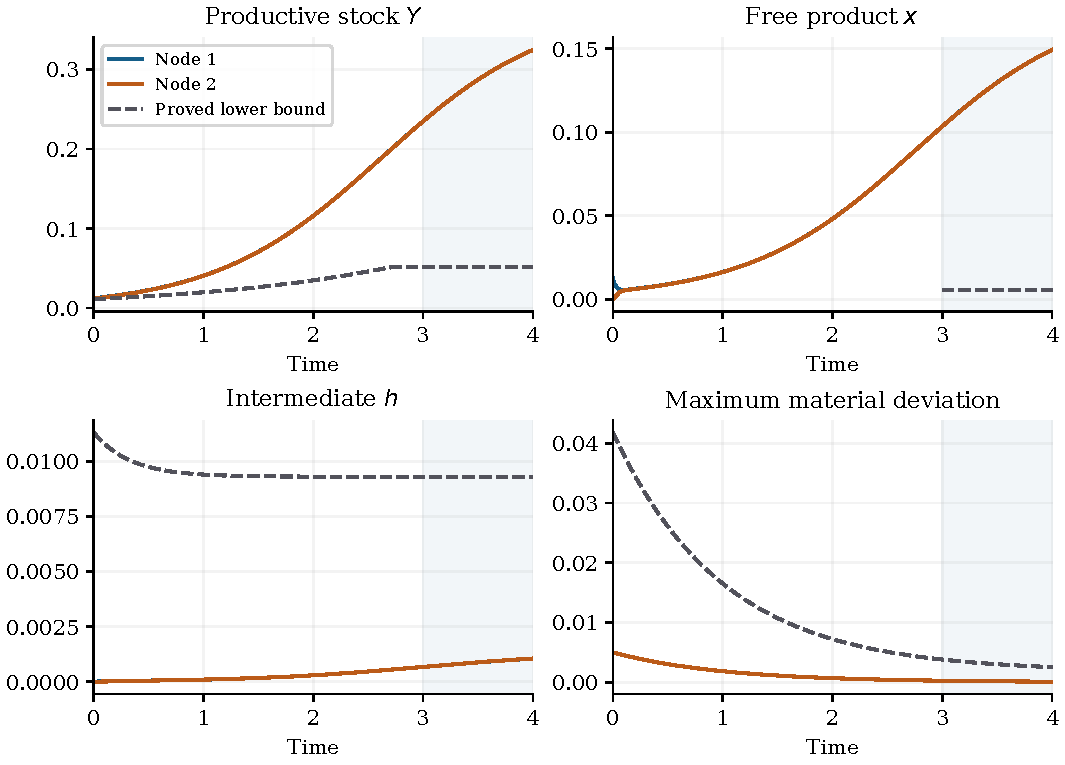
\includegraphics[width=.98\linewidth]{figures/operation.pdf}
\caption{Illustrative deterministic flow for the two-node initial states
\eqref{eq:seeds}, after $q=1/4$, all $\ell_s=0.98$, zero refill error, with
$r_i=20$, $d_i=0.03$ and exchange rate one. Solid curves are numerical trajectories;
dashed curves are the proved pathwise bounds \eqref{eq:matbound}--\eqref{eq:phasebound}.
Shading marks the collection window. The numerical integration is not a stochastic
simulation and supplies no proof evidence. Data and the short integration script accompany
the paper.}\label{fig:operation}
\end{figure}

For the illustrated flow, numerical quadrature gives inventory outputs $0.275164$ and
$0.275162$, free-$X$ outputs $0.128711$ and $0.128710$, and gross service $0.007416$ and
$0.007401$ at nodes one and two. Each food input is $4.75$, including refill. These
normalized deterministic accounts illustrate the separate observables; the stochastic
integer guarantees remain those of Theorem~\ref{thm:mission}.

\subsection{Pulse preparation and history induction}
The categorical pulse moment bound, including floor refill and carried intermediate, gives
preparation failure at most
\begin{equation}
4n e^{-V/100000}+n e^{-V/100000000}.
\end{equation}
For materials the squared-weight sum is at most $(161/80)V$, and for stock
it is at most $(1449/800)V$. The conditional Bernoulli bound proved in
Appendix~\ref{app:donor}, at deviations $V/100$ and $V/4000$, implies these
weakened denominators. The intermediate cannot increase at a pulse, so its
preparation ceiling requires no additional tail. Floor refill costs less than
$1/V$, leaving material error below $0.04$ and stock at least $0.012$.
Each of these pulse and mark exponents dominates the final exponent in
\eqref{eq:mission}. Pulse preparation therefore costs $5n$, and operating noise costs
$14n+10n=24n$, times that exponential. Integration over every pulse outcome gives the
uniform one-cycle failure bound $29n e^{-V/(2\cdot10^{12}(1+\Delta)^3)}$.

Let the history invariant mean that every logged output satisfies \eqref{eq:integer}
and the current state is ready. From an invariant history the physical conditional law
preserves this invariant with probability at least one minus the one-cycle error.
Induction through the unrestricted Markov history kernel loses at most that error per
cycle. Nonnegativity supplies the outer maximum with zero. This proves
Theorem~\ref{thm:mission} without conditioning the law on successful histories.


More explicitly, if $E_j$ denotes success of the first $j$ cycles and
$p=29n\exp[-V/(2\cdot10^{12}(1+\Delta)^3)]\le1$, then
\[
\Law(E_{j+1})=\mathbb E\!\left[\mathbf1_{E_j}
  \Law(\text{next success}\mid\mathcal F_j)\right]
\ge(1-p)\Law(E_j).
\]
Consequently $(1-p)^m\ge1-mp$. For $p>1$ and $m\ge1$ the stated bound is zero;
$m=0$ is immediate. This induction does not assert independent cycles.

\section{Sustained synthesis and resource interpretation}
\begin{proposition}[Augmented-inventory accounting]\label{prop:synthesis}
Let $J(N)=N_X+N_{C_1}+N_{C_2}+2N_Z+N_D$. For each chemical pair $j$ in
Table~\ref{tab:chemistry}, let $H_j$ be its net forward event count over the whole
mission and all nodes, starting just before the first pulse and ending at the last
return. Set $S_J=H_0+H_3-H_6$. Every finite physical path satisfies
\begin{equation}\label{eq:telescope}
S_J=J_{\rm final}-J_{\rm initial}+J_{\rm washout}
       +J_{\rm withdrawn}+J_{\rm pulse\ loss}.
\end{equation}
On a successful $m$-cycle mission with $m\ge1$,
\begin{align}
S_J&\ge nm\lceil V/56\rceil+nV/28-J_{\rm initial}\notag\\
&\ge nV\left(\frac m{56}+\frac1{28}-\frac{161}{160}\right).
\label{eq:synthesis}
\end{align}
The last expression is positive for $m\ge55$ and equals $(913/1120)nV$ for $m=100$.
These consequences hold with the same mission probability lower bound.
\end{proposition}
\begin{proof}
The $J$ increments of the seven forward pairs are $(1,0,0,1,0,0,-1)$;
reverse increments are their negatives. Feed and refill have zero $J$ weight.
Every exchange event cancels globally, and each pulse category removes its actual
inventory weight. Summing these increments proves \eqref{eq:telescope}; nonexplosion
ensures finite event counts. On success, all washout includes the credited inventory
collection, so $J_{\rm washout}\ge nm\lceil V/56\rceil$. Coefficientwise,
$J\ge I\ge5Y/7$, hence $J_{\rm final}\ge nV/28$. Initially $J\le A\le161V/160$
at each node. Discarding nonnegative pulse losses proves \eqref{eq:synthesis}.
Finally the bracket equals $(20m-1087)/1120$, which is positive precisely for
integer $m\ge55$. This is an eventwise consequence, requiring no further probability cost.
\end{proof}
The intermediate is included in the carried inventory but not credited as product.
Thus a long successful mission cannot be explained by draining its initial intermediate
and productive stock. $S_J$ measures net chemical creation of inventory equivalents;
it is not a thermodynamic efficiency or a claim about the identity of atoms in an
experiment. Also $Q_X$ is part of $Q_I$; these outputs must not be added as disjoint products.

In addition to \eqref{eq:yield}, success gives the division-free service inequalities
\[
G\le\frac{56}{5}Q_I,\qquad G\le216Q_X.
\]
They follow from $G\le V/5$, $Q_I\ge V/56$ and $Q_X\ge V/1080$ and sum over
the mission. At fixed $n,V,\Delta$ and failure allowance $0<\delta<1$, a sufficient
mission duration is
\[
m\le\left\lfloor\frac{\delta}{29n}
\exp\!\left(\frac{V}{2\cdot10^{12}(1+\Delta)^3}\right)\right\rfloor,
\]
provided the readiness and $V\ge10000$ conditions hold. A zero right side means
that the certificate supplies no positive mission at this allowance, not certain failure.

\section{A worked operating mission}\label{sec:example}
For the connected example \eqref{eq:seeds}, $n=2$, $m=100$, $\Delta=1$ and
$V=2.24\cdot10^{14}$. The certified success lower bound is
$1-5800e^{-14}\simeq0.9951771334$. On this event the guaranteed total credited
inventory is at least $8\cdot10^{14}$ equivalents, while
\eqref{eq:synthesis} guarantees $S_J\ge3.652\cdot10^{14}$.
The initialization is literal and integral since $V$ is divisible by $20$ and $28$.
The probability guarantee is uniform over the stated controller class.

Figure~\ref{fig:operation} shows the first deterministic cycle with fixed
$r_i=20$, $d_i=0.03$, $q_i=1/4$, $\ell_{is}=0.98$, zero refill error and
exchange rate one. Figure~\ref{fig:cycles} repeats this same pulse from the actual
computed seven-species endpoint for ten cycles, including intermediate carryover.
These coupled deterministic trajectories illustrate the model; the local deterministic
theorem does not by itself certify a deterministic graph extension.
\begin{figure}[ht]
\centering
\includegraphics[width=.96\linewidth]{figures/cycles.pdf}
\caption{Ten deterministic cycles with actual endpoint carryover. Upper panels show
returned stock and intermediate. Lower panels separate collected inventory, collected
free $X$ and gross service (normalized by count scale); each food account is $4.75$
per cycle. Solid curves are numerical results, not a sample of the molecular law.
The accompanying CSV records every node and cycle.}\label{fig:cycles}
\end{figure}
Integration uses Radau with relative tolerance $2\cdot10^{-9}$ and absolute
tolerance $2\cdot10^{-11}$. Product and service integrals are accumulated as additional
ODE coordinates, splitting the flow at the collection boundary. A rerun with both
tolerances reduced by a factor of 100 changes the recorded endpoint and account
values by less than $6\cdot10^{-13}$; neither simulation nor quadrature is proof evidence.

To attach units, choose concentration unit $c_*$ (mol\,L$^{-1}$) and time unit
$\tau$ (seconds). Then $c_{\rm physical}=c_*c$, $t_{\rm physical}=\tau t$ and
\[
V=N_A\Omega c_*,\qquad N_A=6.02214076\cdot10^{23}\ {\rm mol}^{-1},
\]
where $\Omega$ is a reactor's volume in litres. A cycle lasts $4\tau$; a rate-one
washout corresponds to $1/\tau$; each unit feed corresponds to $c_*/\tau$.
A dimensionless second-order coefficient $k$ corresponds to $k/(c_*\tau)$.
At $c_*=1$\,mM the witness scale corresponds to $\Omega\simeq0.372$\,$\mu$L;
at $c_*=1$\,$\mu$M it corresponds to $\Omega\simeq0.372$\,mL.
This conversion is illustrative: no particular $c_*,\tau$, chemical identity,
experimental rates or membrane have been calibrated.

\section{Discussion and verification scope}
The common event is operational: counted effluent, bounded input and transaction
counts, and recovery of the actual state. Material histories make the donor reduction
exact; intermediate storage explains why a naive projection of the refined source
fails. Useful operation can nevertheless be proved without a uniform approximation
of all species trajectories. The synthesis telescope strengthens this interpretation
by accounting for all initially carried intermediate.

For bounded weighted degree, the sufficient per-node count scale grows logarithmically
with node count, mission length and inverse failure allowance. The cubic degree factor
and large numerical constants are features of this sufficient proof. They are not
lower bounds, optimal scaling laws, or a monotonic prediction of how transport changes
physical reliability. The result begins in readiness and concerns finite missions;
it does not assert food-only startup, all-time persistence, arbitrary intermediate
lifetimes, selective or asymmetric transport, asynchronous pulses, or universal
inheritance under reaction refinement.

The refined deterministic theorem, the finite-count mission theorem, its concrete
returned-history construction, the connected witness, and the food-to-output bounds
are supported by Lean proofs. The recorded strict publication verification succeeds
with warnings treated as errors, and the checked declarations report only
\texttt{propext}, \texttt{Classical.choice} and \texttt{Quot.sound}.
The source and dependency hashes were compared with the saved receipt for this paper.
The six-species probability theorem is conventional; selected donor algebra and margins
have separate Lean checks. Propositions~\ref{prop:reduction}, \ref{prop:storage} and
\ref{prop:synthesis}, and the service/duration corollaries, are supplied here as
conventional proofs. We do not describe the entire manuscript as formally verified.

The editable source distribution includes the bibliography, vector figures, numerical
data, reproduction scripts and a claim-to-source map. Formal proof source paths and
the frozen verification environment are identified in that map. The numerical figures
are illustrations of the literal equations and not estimates of stochastic failure rates.

\appendix
\section{Quantitative source estimates}\label{app:estimates}
For completeness, the estimates behind the stock and phase steps can be checked
directly from the displayed chemistry. Put $A_0=A-h$, $B_0=B-h$. If
$A_0,B_0\ge0.9$ and $Y\le0.06$, then
$u\ge119/150$, $w\ge57/70$, $x^2\le(3/50)x$. Expansion of the refined drift gives
\begin{align*}
Y(f)={}&\epsilon_0uw+
 (\tfrac52u-1-d(1+\beta)-\epsilon_0/10)x
 +(\tfrac{11}{2}w-\tfrac{29}{8})c_1\\
&+\tfrac{11}{10}c_2+(r/5-13/5)z-(r/5)x^2+d\beta h/\theta.
\end{align*}
Subtracting $2Y/3$ leaves nonnegative coefficients: the $x$ surplus is at least
$37/1500-d\beta-\epsilon_0/10>0$; those of $c_1,c_2,z$ are at least
$29/280$, $1/6$ and $(r-19)/5$. The count correction contributes $rx/(5V)\ge0$.
Also $I-5Y/7=(2/7)x+(11/56)c_1+(5/7)z\ge0$.

For the matrix $H$ in \eqref{eq:phase}, the first row of its degree-four exponential
polynomial at $1/28$ is
\[
\left(1,\frac{961355}{1229312},\frac{1847785}{1843968},
\frac{665611}{307328}\right).
\]
Dividing by the stock weights gives minimum ratio $961355/1382976$.
The exponential series with a geometric remainder gives
$e^{6/7}\le\sum_{j=0}^7(6/7)^j/j!+(6/7)^8(9/8)/8!\le2357/1000$,
whose square is at most $961355/172872$. Hence multiplying the row by
$e^{-12/7}$ dominates the stock weights divided by eight.
The $x$ loss is bounded by $1+d(1+\beta)+\epsilon_0/10+42(u+x)<48$;
the other diagonal losses are bounded by $43,41,24$. This proves the lower phase
system including the literal duplex propensity.

An alternative conventional derivation of the phase-noise estimate makes its
constant explicit. On a network put $K=\mathcal D\otimes\mathrm{Id}_4+
\mathrm{Id}_n\otimes M$. Then $\|e^{Ks}\|_\infty\le e^{10s}$ and
$\|K\|_\infty\le106+2\Delta$. Integration by parts on a window of length
$1/28$ bounds the common coordinate-noise contribution by
\[
\varepsilon\left[1+e^{10/28}+(106+2\Delta)\int_0^{1/28}e^{10s}\,ds\right]
<8(1+\Delta)\varepsilon.
\]
Here $e^{5/14}<3/2$ and the integral is below $1/20$.
The positive graph semigroup averages the uniform starting stock floor.
This yields \eqref{eq:phasebound}; the formal proof implements the finite adjoint.

For the deterministic theorem the material deviation immediately after the pulse
is below $0.04$ and subsequently decays as $0.04e^{-t}$. The filter ceiling
$h\le1.101\theta$ is invariant: under materials at most $1.1$ its forcing
$x+(\eta_0/\beta)uw<1.101$, so the derivative is negative at the ceiling.
Thus $A_0,B_0>0.9$. Starting at $Y\ge49/4000$, the preceding growth inequality
gives $Y(t)\ge\min\{(49/4000)e^{2t/3},0.06\}$ and hence $Y\ge1/20$ by
$t=5/2$. Material decay and the filter ensure readiness at time four.
The same positive phase system without noise gives at least $Y/8$ in free $x$
after $1/28$ time, which is stronger than the asserted $1/540$ collection floor.
Finally $g\le112201/2500000$, and each food input is $5-q+e\le951/200$.
Integration and recursion prove Theorem~\ref{thm:det} at every fixed admissible $\theta$.

\section{Conventional donor probability proof}\label{app:donor}
The donor uses the same nonexplosion argument and phase matrix. Its stock expansion
is the one above with $-d(1+\beta)x+d\beta h/\theta$ replaced by
$-dx+d\eta_0uw$. The surplus is therefore at least the displayed donor coefficients.
Here are explicit estimates closing its probability proof, without a six-species
instantiation of the refined formal probability root.

For a compensated jump martingale with jumps at most $b/V$ in absolute value and
bracket at time $T$ at most $v/V$,
\begin{equation}\label{eq:elementarytail}
\Law(\sup_{t\le T}|M_t|\ge a)\le
2\exp[-Va^2/(4(v+ba))].
\end{equation}
Indeed $e^u-1-u\le u^2$ for $|u|\le1$ makes
$\exp(\lambda M-\lambda^2\langle M\rangle)$ a nonnegative local
supermartingale when $\lambda b/V\le1$. Localize, apply the crossing bound and
Fatou's lemma, choose $\lambda=Va/[2(v+ba)]$, and repeat for $-M$.
The bound includes the exit jump because brackets use its pre-jump intensity.

Conditional pulse means lie in $[31213/32000,3231/3200]$ for both materials
before floor rounding, and stock mean is at least $49/4000$.
The sums of squared weights are at most $(161/80)V$ and $(1449/800)V$
for material and stock. The centered Bernoulli log-moment bound
$\log\mathbb E e^{\lambda a(B-\mathbb EB)}\le\lambda^2a^2/8$
follows by integrating the tilted variance bound $1/4$ twice.
Applying it at deviations $V/100$ and $V/4000$ gives pulse failure at most
$4ne^{-V/11000}+ne^{-V/15000000}$. On its complement the post-pulse material
error is at most $0.04$ and stock at least $0.012$.

Stop at first material exit from $[0.9,1.1]$, including its jump.
The sum of local propensities divided by $V$ is below $200$, by direct substitution
of the corridor and rate maxima in the six chemical pairs, feeds and washouts.
Coordinate jumps have size at most $2/V$; exchange contributes at most
$2.2\Delta/V$ to each coordinate squared-jump rate. Thus the four-time bracket is
at most $3200(1+\Delta)/V$. Set $\varepsilon_0^*=1/[100000(1+\Delta)]$.
Equation~\eqref{eq:elementarytail} and a union over $6n$ coordinates cost
$12n\exp[-V/(2\cdot10^{14}(1+\Delta)^3)]$.

On this common event, material martingale weights sum to at most eight.
Writing $L=\mathcal D-\mathrm{Id}$, integration by parts gives
\[
A_0(t)-\mathbf1=e^{Lt}(A_0(0)-\mathbf1)+M_A(t)
 +\int_0^t Le^{L(t-s)}M_A(s)\,ds.
\]
Since $\|e^{Lt}\|_\infty\le e^{-t}$ and $\|L\|_\infty\le1+2\Delta$,
the material deviation is at most $0.04e^{-t}+0.00016$. At any first exit this
is strictly below $0.1$, a contradiction, so the stop is removed.
The compensated stock is above
$\min\{0.0119e^{0.6t},0.059\}$: on a sufficiently narrow strip below this
fence, its derivative minus the fence derivative is positive because
$(2/3+2\Delta)(11/2)\varepsilon_0^*\le0.00011$ and the growth surplus is
at least $0.0119/15$. Integrating on a hypothetical downward crossing of the
strip proves comparison. The cap is reached by $11/4$, yielding $Y>0.058$.
The phase estimate above then gives $x>0.007$ on $[3,4]$ and $I>0.04$.
Endpoint material error is below $0.001<1/160$, so readiness returns.

The five stopped marks have jumps at most $2/V$ and brackets at most $9/V$.
Using \eqref{eq:elementarytail} at $a=0.001$, with collection marks gated to
$(3,4]$, costs $10ne^{-V/40000000}$. Actual normalized product is then at least
$0.039$ for $Q_I$ and $0.006$ for $Q_X$. The service compensator is at most
$0.18$, since $d x+d\eta_0uw<0.045$ on the corridor; actual service is at most
$0.181$. Each food account is at most $0.755+4+0.001=4.756$.
These strict inequalities imply all integer ceilings and floors for $V\ge10000$.
The prefactors $5+12+10=27$ give the common one-cycle bound after weakening
exponents. Conditional induction from the actual returned state, as in the main
proof, proves Theorem~\ref{thm:donor}.

\bibliographystyle{plainnat}
\bibliography{references}
\end{document}
